\chapter{Ordinateurs et systèmes}

\begin{multicols}{2}
\section{Le premier ordinateur}


Les ordinateurs tels que nous les connaissons sont des objets qui
s'incrivent dans une longue suite d'inventions et de combinaisons de
technologies diverses.

Si on définit l'ordinateur comme
\begin{quote}
un appareil électronique qui fait des calculs en suivant les
instructions d'un programme enregistré
\end{quote}
le premier ordinateur construit est très probablement le \emph{Manchester
  Small Scale Experimental Machine (SSEM)}\footnote{surnommé ``Baby'', voir \url{http://www.computer50.org/mark1/new.baby.html}},

% http://www.computinghistory.org.uk/userdata/files/1_history-ssem.jpg
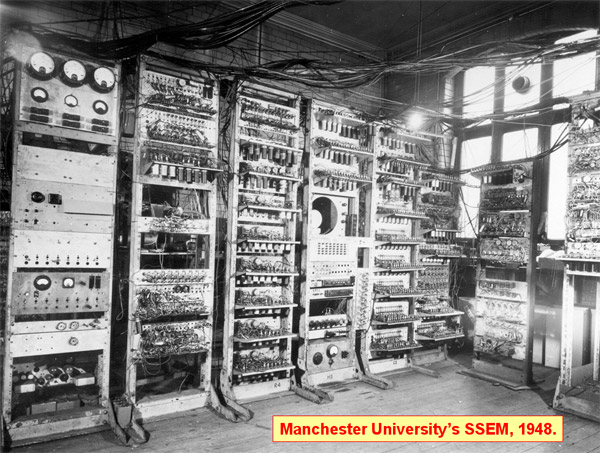
\includegraphics[width=0.9\linewidth]{Historique/1_history-ssem.jpg}

 qui a tourné
pour le première fois le 21 juin 1948. Il avait été réalisé par
Tom Kilburn et Geoff Tootill, dans l'équipe de Freddie Williams,
professeur d'électrotechnique à l'Université de Manchester.

Voir le reportage tourné par la BBC en 1948, sur 
\url{http://news.bbc.co.uk/2/hi/technology/7465115.stm}

\subsection{Les calculateurs électroniques}
\paragraph{Les calculateurs
électroniques à programme} existaient déjà depuis une quinzaine d'années, 
 mais leurs  programmes n'étaient pas
enregistrés en mémoire. Ils étaient soit externes (bande ou carte perforées),
soit figés. Par exemple sur l'ENIAC (1946), des interrupteurs à tourner dans tableau de
connexion pour réaliser les 0 et les 1 d'une mémoire morte. Cette
manière de faire dérivait assez naturellement des machines à traiter
les cartes perforées, utilisées depuis la fin du XIX${e}$ siècle.\footnote{Voir l'article
de Wikipedia consacré à la mécanographie}
%  \url{http://fr.wikipedia.org/wiki/M\%C3\%A9canographie}}.

En réalité le SSEM était un prototype destiné à tester l'utilisabilité
d'une mémoire à tube cathodique inventée par F. Williams. 

\subsection{Mémoire à tube de Williams-Kilburn
}
Cette innovation utilisait un tube d'oscilloscope standard, dans lequel un faisceau
d'électrons permettrait d'allumer des points de phosphore sur l'écran,
avec une certaine rémanence.  Le tube de Williams-Kilburn utilise la propriété
suivante : quand le faisceau bombarde un point de l'écran, des
électrons secondaires sont éjectés par le phosphore, en quantité
différente selon que le point est ou non déjà allumé. En mesurant 
la tension sur une 
plaque métallique devant l'écran, on peut
connaître l'état du point.

% http://www.radiomuseum.org/tubes/tube_williams-kilburn.html
% http://www.radiomuseum.org/forumdata/users/5944/william-kilburn_tube.jpg
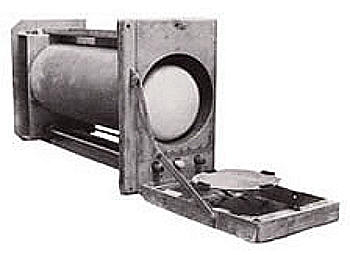
\includegraphics[width=0.9\linewidth]{Historique/william-kilburn_tube.jpg}

En 1947, l'équipe de Williams avait réussi à stocker 2048 bits sur un
écran pendant des heures, ce qui promettait une technologie de mémoire
rapide, bon marché, basée sur des composants standards, destinée aux calculateurs. 

L'idée est donc venue assez naturellement de fabriquer un calculateur
simple avec une mémoire à tube pour en tester la fiabilité dans une
machine qui effectue plusieurs milliers de lectures/écritures par
seconde. Jusque là, le tube avait été testé en adressant les bits par
un jeu d'interrupteurs manuels...

\subsection{Architecture et programmation}

\paragraph{L'architecture du SSEM} est très simple. En termes modernes,
c'est une machine 32 bits, avec une mémoire de 32 mots de 32 bits
(1024 bits stockés sur un tube), extensible à 8192. 

Les calculs se
font en nombre entiers en notation complément à deux.

Deux tubes étaient utilisés pour les registres spéciaux :
\begin{itemize}
\item l'un pour l'accumulateur A (32 bits) 
sur lequel se font les opérations
\item l'autre pour CI (control instruction) qui contient d'adresse de
  l'instruction en cours, et PI (present instruction), l'instruction
  elle-même
\end{itemize}
Un dernier tube (sans plaque) dupliquait le premier, permettant de
voir les bits en mémoire\footnote{les bits de poids fort sont à droite, contrairement à la notation habituelle des nombres en binaire}.

\begin{center}
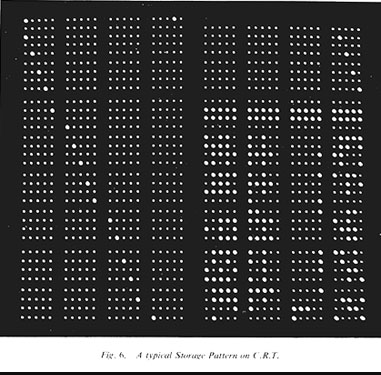
\includegraphics[width=0.6\linewidth]{Historique/crt.jpg}
% http://www.computer50.org/mark1/pictures/crt.jpg
\\
La mémoire du SSEM
\end{center}

\paragraph{Le jeu d'instructions} était réduit à 7 instructions d'un 
format unique : 
3 bits pour le code opération, et 13 bits pour l'adresse S de
l'opérande. les 16 derniers bits étaient inutilisés. Les 7 opérations
étaient

\begin{itemize}
\item \texttt{LDN S} (load negative) \verb/A = - Mem[S]/, qui charge
  dans l'accumulateur l'opposé du contenu d'un mot mémoire
\item \texttt{SUB S} (subtract) \verb/ A = A - Mem[S]/, qui soustrait
  le contenu d'un mot
\item \texttt{STO S} (store) \verb/ Mem[S] = A/, qui copie en mémoire
  le contenu de l'accumulateur
\item \texttt{CMP} (compare) \verb/ If A < 0, CI = CI + 1/, qui saute
  l'instruction suivante si l'accumulateur est négatif,
\item \texttt{JMP S} (jump) \verb/ CI = Mem[S] + 1/, qui provoque un
  saut indirect, à l'adresse contenue dans un mot de la mémoire.
\item \texttt{JRP S} (jump relative) \verb/ CI = CI + Mem[S] + 1/,
  pour un saut indirect relatif.
\item  \texttt{HLT} (halt) qui arrête l'ordinateur.
\end{itemize}

Ce jeu d'instruction a été choisi parce qu'il était réalisable avec un
minimum de circuits électroniques. Il ne simplifie évidemment pas la
vie du programmeur.  Par exemple, pour additionner deux nombres x et y
situés aux adresses 20 et 21, il faut 4 opérations en passant par une
variable temporaire (d'adresse 22)
\begin{verbatim}
0   LDN  20  ; A contient -x
1   SUB  21  ; A contient -x-y
2   STO  22  ; Mem[22] contient -x-y
3   LDN  22  ; A contient -(-x-y) = x+y
\end{verbatim}

Voici un exemple plus complexe, écrit en utilisant
des adresses symboliques : le calcul du maximum de
deux nombres X et Y et le rangement dans Z.


\begin{verbatim}
# calculer la différence

0   LDN   X   ; A = -x
1   STO   TMP ; TMP = -x
2   LDN   TMP   ; A = x
3   SUB   Y

# selon la différence, charger -X ou -Y 
# dans l'accumulateur

4   CMP  
5   JMP   I8 ; si A positif
6   LDN   Y
7   JMP   I9
8   LDN   X

# et envoyer l'opposé de l'accumulateur dans Z

9   STO   TMP
10  LDN   TMP
11  STO   Z
12  HLT

# Les variables

13 X   = 42
14 Y   = 15 
15 TMP = 0
16 Z   = 0

# les adresses de saut
17 i8    = 7 
18 i9    = 8
\end{verbatim}

Remarque : pour aller à l'instruction 9, l'instruction 7 charge le mot
d'adresse 17 dans le CI, auquel il ajoute 1 comme après toute
instruction.  C'est pourquoi le mot 17 contient 8, l'adresse qui
précède celle de l'endroit où le programme doit se poursuivre.



\subsection{Une démontration probante}

Le programme précédent suffit à occuper plus de la moitié de la
mémoire disponible sur le SSEM, qui n'a évidemment jamais servi à
faire des calculs très complexes. Le clou du spectacle était un
programme de 17 instructions\footnote{La légende de l'université de
  Manchester dit que c'est le seul programme que le professeur
  Williams ait jamais écrit.}  pour trouver le plus grand diviseur
propre d'un nombre N, en essayant de le diviser successivement par
N-1, N-2 etc., la division étant elle-même réalisée par soustraction
successives.

% http://www.oldcomputers.arcula.co.uk/files/images/hist409t.jpg
\begin{center}
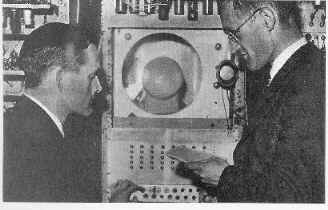
\includegraphics[width=0.9\linewidth]{Historique/hist409t.jpg}
\\
Kilburn et Williams devant la console du SSEM
\end{center}

Il a fallu 52 minutes de calcul (et 3,5 millions d'opérations) pour
établir que le plus grand facteur propre de $2^{18}$ était
$2^{17}$. Ce que tout le monde savait déjà évidemment. Sur
  l'écran phosphorescent, une puissance de deux est facile à lire : un
  point allumé sur une ligne éteinte. 

Peu importe : l'objectif était de montrer que
la mémoire était fiable : peu importe les calculs du moment que le
résultat est correct après des millions d'opérations.

\subsection{Les suites}

Un vrai ordinateur est sorti de ces travaux, \emph{Manchester
Automatic Digital Machine} (MADM), opérationnel en avril 1949, et qui a
donné naissance aux machines du constructeur Ferranti.

Quant aux tubes de Williams, ils ont été utilisés comme mémoires dans
quelques ordinateurs célèbres (UNIVAC 1103, Whirlwind, IBM 701, IBM
702 ...) avant d'être rapidement supplantés par les mémoires à tores
de ferrite, qui ont dominé le marché pendant 20 ans de 1955 à 1975,
avant d'être remplacées par les mémoires à semi-conducteurs que nous
utilisons aujourd'hui.

\section{Structure d'un ordinateur simple}

Schématiqument, un ordinateur est composé
\begin{itemize}
\item d'un \textbf{processeur}, circuit électronique capable d'exécuter une à
  une (mais très vite) les instructions d'un programme
\item d'une \textbf{mémoire centrale}, circuit qui sert à mémoriser les données
  et les programmes pendant leur exécution
\item des \textbf{périphériques} : imprimante, carte réseau, carte graphique, disque dur
  etc. reliés par des contrôleurs d'interface.
\end{itemize}

Le rôle du Baby étant de tester la fiabilité des mémoires à tubes de
Williams-Kilburn, il était dépourvu de périphérique. 

Dans ce chapitre, nous présentons ces divers éléments de façon très
simplifiée.


\subsection{La mémoire}

Différentes technologies ont été utilisées pour réaliser
les mémoires des ordinateurs : bascules bistables à base 
de tubes (triodes),
mémoires à tores de ferrite, à transistors,  
circuits intégrés etc.

Indépendamment des technologies, la mémoire est un organe
qui a pour fonction de stocker et restituer des ``mots binaires''
repérés par une \texttt{adresse}.

Les mots sont de taille fixe\footnote{Il y a eu bien sûr quelques
  exceptions, qui ont été des échecs. Dans l'histoire des ordinateurs,
  beaucoup de choses ont été essayées.}, par exemple l'ATLAS (réalisé
en 1962 conjointement par l'université de Manchester, Ferranti et
Plessey) avait une mémoire de 16384 mots de 48 bits.  Les
micro-processeurs des années 70 étaient souvent des machines à octets
(mot = 8 bits), de nos jours ce sont des mots de 32 ou 64 bits.

La mémoire communique avec le reste de l'ordinateur par
3 bus (groupes de fils)
\begin{itemize}
\item le \textbf{bus de contrôle} (il faudrait dire bus de commande), 
qui indique à la mémoire l'opération 
que l'on veut effectuer : lecture ou écriture ;
\item le \textbf{bus de données}, bidirectionnel, qui sert à émettre et
recevoir les mots ;
\item le \textbf{bus d'adresses}, qui indique à la mémoire l'adresse
concernée.
\end{itemize}

\FIGURE{mod-initial.png}{La mémoire et ses trois bus}

\paragraph{Opérations :}
\begin{itemize}
\item lecture : pour consulter l'adresse A en  mémoire, 
le processeur
place le nombre A sur le bus d'adresses, et envoie le 
signal de contrôle ``lecture''. Après un petit délai de réponse, 
le contenu du mot d'adresse A est présent sur le bus de données.
\item écriture : pour envoyer un mot M à l'adresse A, le processeur
place A sur le bus d'adresses, M sur le bus de données et
active l'ordre d'écriture.
\end{itemize}

\paragraph{Remarque :}  sur certaines machines (c'était le cas du 
processeur 8088 qui équipait les premiers PC d'IBM\footnote{Le
  processeur 8086 d'INTEL possédait des bus séparés, le 8088 qui en
  était dérivé était à la fois plus cher à fabriquer (c'est un 8086
  avec en plus des circuits de multiplexage/démultiplexage) et moins
  performant. Ceci dit, le 8086 nécessitait une famille de circuits
  associés 16 bits (contrôleurs d'interruption, etc), alors que le
  8088 pouvait se contenter des circuits 8 bits qui étaient déjà
  produits en masse pour les microprocesseurs 8080 et 8085 qui
  équipaient les micro-ordinateurs les plus courants de l'époque (sous
  CP/M).}), les bus de données et d'adresses sont \emph{multiplexés},
ils partagent des fils. L'avantage est de minimiser le nombre de
connexions entre circuits intégrés (et du nombre de pattes ),
l'inconvénient est que les données et les adresses ne sont pas être
transmis en même temps, ce qui se fait au détriment des performances.
Un signal de commande supplémentaire précise si l'information qui
circule est une adresse ou une donnée.

\subsection{Le processeur}

Un processeur est un dispositif électronique relativement simple, composé
de circuits logiques divers.  Il communique avec la mémoire (voir plus haut)
et les périphériques par des bus de données, d'adresses, et de commande.

Son rôle est d'exécuter, les unes après les autres, des instructions
qui sont stockées en mémoire.

\subsubsection{Instructions et registres}

Le \textbf{compteur de programme}\footnote{ou pointeur 
d'instruction, compteur ordinal...} est un registre\footnote{en électronique numérique, un \emph{registre}
est un circuit qui mémorise quelques bits d'information. Il est possible d'y 
charger une valeur, et de la relire ensuite.
} qui contient l'adresse de la prochaine
instruction à exécuter.  C'est un \emph{compteur} parce que, la plupart
 du temps, on va lui ajouter 1 pour passer à l'instruction suivante.

La première action du processeur est de lire en mémoire le mot qui
contient cette instruction, et de la placer dans un \textbf{registre
  d'instruction}, où il sera décodé.\footnote{La terminologie du SSEM
les désignait par  CI (current instruction) et PI (present instruction)}.

Par exemple, on aura peut être lu le mot de 32 bits
\textbf{000110000100001100000000000101010}
qui, sur un PowerPC 32 bits, se décompose en
\textbf{001110 00010 00011 00000000 000101010}
ce qui représente
\begin{itemize}
\item les 6 premiers bits : le code de l'opération ``ajouter une constante''
\item un numéro de registre destination (registre 2) sur 5 bits
\item un numéro de registre source (registre 3)
\item une constante (42) codée sur 16 bits
\end{itemize}
et qui signifie : ajoutez au registre de travail numéro 3 la valeur 42, 
et placez le résultat dans le registre 2, ce qu'on écrirait en 
\emph{langage 
d'assemblage} 
\begin{verbatim}
	  addi  2,3,42
\end{verbatim}

L'exécution de l'opération ci-dessus fera appel à différents autres circuits
\begin{itemize}
\item les \textbf{registres généraux}, qui stockent des valeurs intermédiaires
(il y en a 32 sur le PowerPC). C'est la généralisation de l'accumulateur A
du SSEM.
\item une \textbf{unité arithmétique}, qui sera ici chargée de
  s'occuper de l'addition.
\end{itemize}

Certaines opérations permettront des transferts entre registres et mémoire, 
par exemple
\begin{verbatim}
   stw  5,0,1234
\end{verbatim}
envoie (\emph{store}) le contenu du registre général 5 à l'adresse
1234 de la mémoire.

Il y a également des instructions pour comparer le contenu de registres,
et d'autres qui changent le cours de l'exécution si une condition
est remplie, en indiquant le numéro de la prochaine instruction à exécuter.

En fait, les instructions de comparaison positionnent
des indicateurs booléens dans un \textbf{registre de condition}
qui mémorisent le résultat de la comparaison 
(inférieur, supérieur, égal ?)

En fonction de ces indicateurs, les \textbf{instructions de branchement 
conditionnel} incrémentent le compteur de programme, ou lui affectent 
une autre adresse.

Rappel : sur le SSEM, le bit de signe de l'accumulateur était l'unique
indicateur de condition, utilisé par l'instruction \texttt{CMP}.

À ces opérations s'ajoutent des \textbf{instructions d'entrée-sortie},
permettant le dialogue avec des circuits \textbf{contrôleurs de
  périphériques}, ainsi que des instructions spéciales que nous
verrons plus tard.


Tous ces circuits fonctionnent sous le contrôle d'un \textbf{séquenceur},
qui enchaîne les différentes étapes :
\begin{itemize}
\item envoyer le contenu du PC sur le bus d'adresse, et un ordre de lecture
\item copier la valeur présente sur le bus de données dans le registre
  d'instruction RI, et indiquer la fin de lecture
\item décoder l'instruction contenue dans le RI
\item l'exécuter. Si il s'agit de ``ajouter 42 au registre 3'' :
\begin{itemize}
\item envoyer le contenu du registre 3, la valeur 42 et l'ordre d'addition
l l'unité arithmétique (circuit de calcul)
\item copier le résultat dans le registre 3
\item ajouter 1 au PC
\end{itemize}
\item et recommencer
\end{itemize}

\end{multicols}
\subsubsection{Architecture interne d'un processeur}
% http://upload.wikimedia.org/wikipedia/commons/5/5d/Intel_8080_arch.svg

Le schéma ci-dessous montre l'architecture interne du processeur 8080
mis sur le marché par Intel en Avril 1974. C'est le second
micro-processeur 8 bit, après le 8008.

\begin{center}
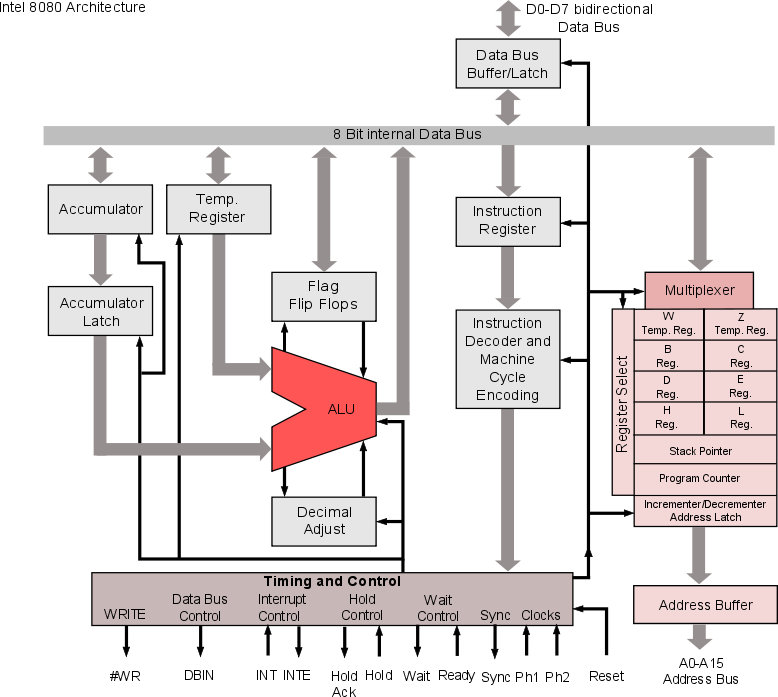
\includegraphics[width=\linewidth]{Historique/8080.png}
\end{center}

On retrouve 
\begin{itemize}
\item en haut, le bus de données de 8 bits
\item en bas à droite le bus d'adresse 16 bits,
\item à gauche l'accumulateur A
\item au centre l'unité arithmétique et logique (ALU)
\item le registre d'instruction
\item à droite une ``banque de registres'', dont le compteur de programme,
et des registres de travail (B,C,D ...)
\end{itemize}

\begin{multicols}{2}

\subsubsection{Le modèle du programmeur}

Dans un ordinateur, certains registres sont utilisable directement par le
programmeur (comme le registre accumulateur par exemple), et d'autres ont
un rôle interne (le registre d'instruction).

Ce qu'on appelle \textbf{modèle du programmeur}, c'est la partie
qui est utilisable directement par le programmeur
\begin{itemize}
\item le compteur de programme,
\item les registres généraux et spécialisés
\item les registres de condition
\item les différentes catégories d'instruction
\begin{itemize}
\item chargement/ rangement en mémoire
\item arithmétique
\item logique : et, ou, décalages...
\item tests
\item branchements conditionnels et inconditionnels,
\item ...
\end{itemize}
\end{itemize}

Par exemple, dans le 8080, le registre C est utilisable comme opérande
d'une instruction, par exemple \texttt{MOV A,C} (copie de C dans A),
il fait donc partir du modèle contrairement au registre TEMP qui sert
d'intermédiaire dans certaines instructions. Par exemple l'instruction
\texttt{ADD B} (ajouter le contenu du registre B à l'accumulateur) se
déroule en deux temps
\begin{enumerate}
\item copier B dans TEMP, 
et A dans le registre ``latch'' (autre registre temporaire), pour les présenter en entrée de l'UAL,
\item envoyer le résultat de LATCH+TEMP, sortant de l'UAL, dans A.
\end{enumerate}

\begin{exercice}
Pourquoi y a-t-il deux étapes, et non une seule ?
\end{exercice}


\subsubsection{La programmation en langage machine}

Un exemple de programme en pseudo-assembleur  vous montre
le niveau de détail auquel il faut descendre quand on programme
dans un \emph{langage machine} : la séquence ci dessous, 
qui commence à l'adresse 100, 
calcule la somme des entiers de 1 à N, en supposant que N est dans le registre 3
et que le résultat doit aller dans le registre 4. 
\begin{verbatim}
100	   mettre la valeur 0 dans r4 
101	   comparer r3 et la valeur 0
102	   si égal, aller à 106
103	   ajouter r3 à r4
104	   ajouter la valeur -1 à r3
105	   aller à 101
106    ...
\end{verbatim}

Après l'exécution de l'instruction d'adresse 102, le compteur de programme
vaudra 103 ou 106, selon la valeur des indicateurs 
positionnés par l'instruction précédente (101).

\begin{exercice}
Écrivez un programme du même type pour le SSEM, en essayant de le
faire tenir sur 32 mots.
\end{exercice}

Comme vous le voyez, un processeur n'est pas bien compliqué. C'est un
assemblage de quelques circuits de base : registres, additionneurs,
etc. qui sait exécuter des instructions de base très élémentaires.

Ce qui est compliqué c'est de combiner des instructions aussi
rudimentaires pour effectuer des traitements utiles (qui ne sont pas
forcément simples, eux). Affronter cette complexité, c'est la
spécificité du travail du programmeur.

\subsection{Les périphériques}

Enfin, dès les années 60, une grande variété de périphériques permet
l'entrée, la sortie et le stockage des données, ainsi que la
communication.

Sur les premiers ordinateurs, les périphériques courants étaient
\begin{itemize}
\item les lecteurs de rubans perforés, support fragile et peu commode
  hérité des téléscripteurs, abandonnés rapidement.
\item Les lecteurs et perforateurs de cartes (hérités de la mécanographie),
\item les imprimantes;
\item les lecteurs de bandes magnétiques. 
\item des terminaux interactifs : machines à écrire électriques, voire
  écrans cathodiques.
\end{itemize}

Assez rapidement, on en est venu à utiliser un petit ordinateur
auxiliaire - dit ``frontal'' - pour recopier les cartes perforées sur
des bandes magnétiques, de lecture bien plus rapide. Et inversement,
les résultats de l'ordinateur principal étaient transférés sur des
bandes magnétiques que le frontal se chargeait de faire
imprimer ou perforer.

Ainsi on économisait le temps précieux du gros ordinateur.

\subsection{Les outils de programmation}

Dans les premiers temps de l'informatique, le programmeur écrivait ses
programmes en binaire, en utilisant la liste des instructions de
l'ordinateur (instruction set) et en les codant lui même en binaire.
Pour des programmes de quelques dizaines d'instructions, c'était
encore envisageable.

Il est ensuite apparu que cette activité de codage, éminemment fastidieuse,
était trop sujette à erreurs. Il était donc préférable d'utiliser 
un programme  pour faire mécaniquement ce codage sans risque d'erreur. 

L'histoire officielle dit que l'idée d'utiliser un programme de
traduction vient de John Neumann en 1945, mais selon d'autres
sources\footnote{\url{https://beacon.salemstate.edu/~tevans/VonNeuma.htm}},
Von Neumann était en fait initialement opposé à cette idée (émise par
un étudiant), parce que cela gaspillait le précieux temps de calcul de
l'ordinateur, alors qu'on pouvait très bien confier ce travail à
des étudiants modestement rémunérés.

Un programme écrit en \emph{langage d'assemblage} se présente comme
une suite d'instructions utilisant les codes mnémoniques, comme
\texttt{addi} pour ``add immediate value'' sur le PowerPC. Parfois
c'est plus obscur, comme \texttt{lwzxu} (load word with zero indexed
with update). L'\emph{assembleur} est le programme de
traduction\footnote{mais on dit souvent, par métonymie,
``programmer en assembleur''}, qui assemble les traductions de
chaque instruction.

On est ensuite passé (au milieu des années 50) à la traduction
automatique de formules mathématiques, puis de programmes complets,
avec le langage FORTRAN (Formula translator). Là aussi, l'intérêt
n'était pas évident pour tout le monde. Le même John Von Neumann a
déclaré, quand on lui a présenté FORTRAN en 1954 « why would you want
  more than machine language ? »

Inversement, l'arrivée de langages de haut niveau a parfois soulevé
un enthousiame excessif.  En effet, il suffisait d'écrire
\begin{lstlisting}
       multiply PRIX-UNITAIRE 
             by QUANTITE giving  PRIX.
       add PRIX to TOTAL.
\end{lstlisting}
là où, autrefois, un professionnel barbu grassement rémunéré
produisait des  lignes de code absolument incompréhensibles
\begin{lstlisting}
       load  PU
       mult  QTE
       store PRIX
       add   TOT
       store TOT
\end{lstlisting}
y compris par son chef de service, incapable d'en vérifier la qualité.

Quand COBOL a été annoncé au début des années 60, certains y ont vu,
un peu vite, la fin du métier de programmeur.

C'était en effet la fin d'un certain type de programmation, mais il
reste que même si le code est écrit avec des phrases anglaises et
semble facile à relire après une formation d'une semaine, la
difficulté est en réalité dans l'algorithmique et dans l'organisation
du code, composé d'une multitude d'opérations simples.  La
programmation reste un métier à part entière, qui ne s'improvise pas.

\section{Utilisation en mono-tâche}

Les faibles capacités des premiers ordinateurs (quelques dizaines de
kilo-octets de mémoire) ne permettaient que de faire exécuter un
programme à la fois.

Un opérateur était donc chargé de mettre le travail fourni par les
utilisateurs (cartes perforées ou bande magnétique) dans la mémoire de
la machine, de lancer l'exécution et de récupérer les résultats
imprimés (ou enregistrer). Et de recommencer avec le travail suivant.

Chaque travail disposait donc de l'intégralité des ressources de la
machine.

 \begin{exercice}
Les premières machines, expérimentales,
étaient utilisées en mono-tâche à la demande. Quand un utilisateur
arrivait avec un travail à faire passer sur le calculateur, il devait
attendre que les précédents aient libéré la place avant d'utiliser la
machine.

Imaginons l'arrivée de 4 utilisateurs : 
\begin {itemize}
\item John arrive à 8h00, avec un travail qui dure 40 mn
\item Grace arrive à 8h10, avec un travail de 30 mn
\item Alan arrive à 8h20, avec un travail de 1 h 5 mn
\item Niklaus arrive à 8h40, avec un travail de 25 mn
\end {itemize}

\begin{enumerate}
\item
Quel est le ``temps de service'' pour chaque utilisateur (durée entre
son arrivée en salle d'attente et la fin de son travail), si ils
passent dans l'ordre d'arrivée (politique FIFO, \emph{first-in first-out}) ? Calculez le
temps de service moyen.
\item
Mêmes questions si les utilisateurs décident de faire  passer en premier
celui  qui\footnote{parmi
  ceux qui sont présents} a le travail le plus court (politique dite ``du plus cours temps d'exécution'').
\end{enumerate}
\end{exercice}

\subsection{Moniteur d'enchaînement des travaux}

Pour éviter de perdre du temps, on a vite eu l'idée d'automatiser
l'enchaînement des travaux. Un petit programme, toujours présent en
mémoire, assurait la lecture du travail suivant dès qu'un travail
était terminé, et gagnait ainsi de précieuses minutes.

Cet embryon de système peut prendre la forme d'une boucle de quelques
instructions pour copier en mémoire les cartes de l'exécutable à
charger, avant de lui transférer le contrôle.  Un programme
utilisateur qui se termine normalement doit simplement relancer le
moniteur.

En début de journée (et après chaque crash), l'opérateur manipule les
interrupteurs de la console pour entrer ce ``chargeur'' en mémoire.
Dans une version plus élaborée, c'est un dispositif électronique qui lit
un ruban perforé contenant le chargeur : il suffit d'appuyer sur un bouton
pour ``recharger le chargeur''.

Encore mieux : le programme sur bande perforée peut servir à charger
un système plus volumineux, depuis un autre périphérique plus rapide
(bande, disque ou tambour magnétique). C'est ce qu'on appelle le
\textbf{bootstrapping}, ou \textbf{amorçage} : la procédure de
démarrage d'un ordinateur, qui comporte notamment le chargement du
programme initial, et qui peut se faire en plusieurs étapes.

Ce programme résident comportait aussi des sous-programmes (par
exemple lecture-écriture sur bande magnétique, sur disque etc.) qui
pouvaient être appelés par les programmes des utilisateurs, et qu'il
n'était donc pas nécessaire de recharger avec chaque travail.


\subsection{Planification de travaux}

Dans les entreprises, des informaticiens étaient chargés de la
planification de l'exploitation : un certain nombre de travaux
devaient ``passer'' sur l'ordinateur, à eux de décider quand et dans
quel ordre, en tenant compte de diverses contraintes :
\begin{itemize}
\item la taille mémoire de chaque programme, et celle de la machine,
\item les périphériques utilisés : sur une installation à 3 lecteurs
  de bandes, on ne peut pas faire tourner en même temps 2 programmes
  qui ont chacun besoin de 2 lecteurs.
\item les priorités définies par l'entreprise\footnote{Du moins
  présentées comme telles par le Directeur Informatique, qui trouve là
  un moyen d'asseoir sa position stratégique dans l'entreprise en négociant
sa collaboration avec d'autres Directeurs..}
\end{itemize}
et en optimisant à la fois la satisfaction de chaque service
demandeur, et la rentabilisation des matériels.

\begin{exercice}
Soit une installation avec un ordinateur mono-tâche.  A partir de 8h00,
on doit faire passer trois travaux A, B, C qui durent respectivement
1h, 30 min, et 45min.  Et les utilisateurs sont évidemment pressés
d'obtenir les résultats.

Quel est le temps d'attente moyen des utilisateurs si on les fait
passer dans cet ordre sur l'ordinateur (mono-tâche).  Dans l'ordre
inverse ?  Quel est l'ordre optimal ?
\end{exercice}


\subsection{Modifications matérielles nécessaires}

Malheureusement, la coexistence en mémoire du ``superviseur'' et du travail
utilisateur introduit de nouveaux problèmes. En effet, un programme
utilisateur ``buggé'' (intentionnellement ou pas) peut
\begin{itemize}
\item altérer la partie de la mémoire réservée au superviseur,
  conduisant au plantage de la machine
\item utiliser de façon incorrecte les instructions d'entrés-sorties
  (accès illégaux à des fichiers, périphériques endommagés, etc.)
\end{itemize}

Ceci a conduit à quelques modifications du processeur, suggérées dès la fin des années 50
\begin{itemize}
\item le processeur possède deux modes de fonctionnement ``maître'' (ou superviseur, ou privilégié) et le mode ``esclave'' (normal). Ceci est matérialisé
par une bascule 1 bit.
\begin{itemize}
\item le superviseur s'exécute en mode maître, et les programmes utilisateurs en mode esclave.
\item en mode maître, le processeur a accès à toute la mémoire, et
  peut exécuter toutes les instructions de la machine.
\item en mode esclave, la zone mémoire accessible par le processeur
  est restreinte : deux registres indiquent le début de cette zone, et
  sont constamment comparés avec le compteur ordinal.
\item en mode esclave, certaines instructions (par exemple les
  instructions d'entrée-sortie directes) ne peuvent par être
  exécutées\footnote{Dans le Stretch d'IBM, les ingénieurs avaient oublié
    de rendre privilégiée l'instruction qui permet de passer en mode
    maître. Doh! }.
\end{itemize}
\item Quand un programme viole ces règles d'accès, une
  \textbf{exception} se produit : le contrôle est rendu au
  superviseur, à une adresse fixée au départ. Le superviseur examine
  donc la situation et décide des suites à donner (reprendre le
  programme, y mettre fin etc).
\item pour appeler les sous-programmes du superviseur, un programme
  utilise une instruction spéciale (``syscall'', trap logiciel, ...),
  qui provoque aussi une exception. Le superviseur se charge alors
  d'effectuer (en mode privilégié) l'opération demandée, avant de
  rendre la main au programme appelant.
\item Quand une exception se produit, le contenu du compteur de programme
est automatiquement sauvegardé, soit dans une pile en mémoire,
soit dans un registre spécial. Ceci permet de reprendre éventuellement 
l'exécution
là où elle en était arrêtée
\end{itemize}

\subsection{Déroulement d'un appel système}

\paragraph{Point de vue du programmeur d'application}

Par exemple, sous MS-DOS, pour faire afficher une chaîne de caractères il
fallait
\begin{itemize}
\item placer le nombre 9 dans le registre AH
\item placer l'adresse de la chaîne dans la paire de registres DS:DX
\item appeler l'instruction  \texttt{INT 21H}
\end{itemize}


\paragraph{Déroulement} L'exécution de l'interruption 33 (21H)
déclenche l'appel au système d'exploitation, dans la \textbf{ routine
  de traitement de l'interruption 21H}. Ce sous programme consulte le
registre AH qui indique la fonction demandée : 9 = affichage d'une
chaîne. Une fois cette fonction affectée (par copie de caractères
dans la mémoire de l'écran), le système place le code de retour 24H
(36) dans le registre AL, et rend la main au programme utilisateur.


\section{Profiter des temps morts : la multiprogrammation}

\subsection{Motivation économique}

A l'époque (début des années 60) les ordinateurs coûtent une fortune,
 on essaie donc de les rentabiliser au maximum.

Les machines sont composées d'une unité centrale (processeur et
mémoire) et de périphériques : lecteurs de cartes perforées, de
bandes, imprimantes etc.
Or on observe que les opérations d'entrées-sorties sont extrêmement
lentes par rapport aux possibilités d'un processeur.

Prenons par exemple le Gamma 60 dont le premier exemplaire a été livré
par la société Bull à la SNCF en 1958, avec 6 imprimantes et 16 dérouleurs
de bande, il occupait $360 m^2$.

\begin{center}
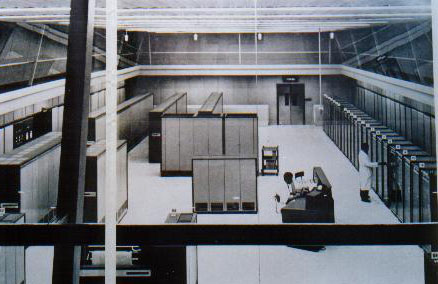
\includegraphics[width=\linewidth]{Historique/Gama2_60.jpg} \\
source : \url{http://histoireinform.com/Histoire/+infos2/chr4infa.htm}
\end{center}

Pour les périphériques : 
\begin{itemize}
\item le lecteur de ruban fonctionnait à 300 caractères par seconde
\item les cartes perforées de 80 colonnes étaient lues à 300 cartes/mn
\item les imprimantes fonctionnaient à 300 lignes par minute
\end{itemize}

et une instruction (opération sur nombres de 10 chiffres) prenait de
100 à 500 microsecondes, soit des dizaines de milliers par seconde.


Dans ces conditions, il est clair que le processeur est le plus souvent
en attente d'une E/S.

L'idée est donc de faire cohabiter plusieurs tâches dans
la mémoire : quand la tâche ``active'' demande à lire des cartes sur
le lecteur, on met à profit le temps libre du processeur pour faire
avancer une autre tâche.

\end{multicols}

\subsection{Étude d'un cas}

Imaginons deux tâches A et B: 
\begin{itemize}
\item la chargement de A  depuis le lecteur de cartes dure 20 secondes, elle fait du calcul pendant 30 secondes, et l'impression des
résultats prend 1 minute ;
\item le chargement de la seconde B dure  10 secondes, son calcul 20 secondes et l'impression 30 secondes.
\end{itemize}


\begin{multicols}{2}

Le graphique ci-contre montre ce qui se passe sous le contrôle d'un ``moniteur
d'enchaînement de travaux''. La tâche B n'est chargée en mémoire que
quand A s'est terminée ($t=110 s$) et se termine à $t=170 s$.

Le processeur a travaillé $30 + 20 = 50s$, soit un taux d'occupation de 
$50/170 = 29,4 \%$.
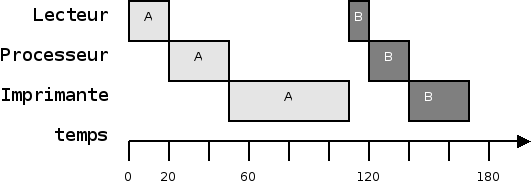
\includegraphics[width=.95\linewidth]{memoire-images/exemple-multitache-1.png}

\end{multicols}

\begin{exercice}
\begin{itemize}
\item calculez le taux d'occupation du lecteur de cartes
\item calculez le taux d'occupation de l'imprimante.
\end{itemize}
\end{exercice}

\begin{multicols}{2}
Voici maintenant le déroulement dans un système multitâche ; la tâche B est
chargée dès que le lecteur a été libéré, puis est exécutée quand le processeur
est libre, etc.
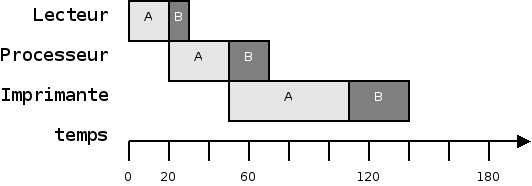
\includegraphics[width=.95\linewidth]{memoire-images/exemple-multitache-2.png}
\end{multicols}

\begin{exercice}
\begin{itemize}
\item Calculez les taux d'occupation, comparez avec les chiffres précédents.
\item Même question si on commence par exécuter B au lieu de A.
\item Imaginons qu'il s'y ajoute une troisième tâche C semblable à B. Représentez 
le déroulement dans les deux cas (enchaînement séquentiel et multitâche). Comparez les chiffres.
\end{itemize}
\end{exercice}

\begin{multicols}{2}

\subsection{La mise en oeuvre du multitâche}

Pour mettre en oeuvre efficacement le multitâche, il faut
que le processeur ne soit pas bloqué en attente des opérations d'entrée-sorties, qui 
doivent se dérouler en parallèle avec les calculs.

On confie donc le pilotage de périphériques à des circuits
spécialisés, à qui le processeur enverra des commandes (requêtes
d'E/S), et qui préviendront le processeur, par un \textbf{signal
  d'interruption}, quand la requête est terminée.  Les interruptions
sont traitées comme les exceptions vues plus haut.

Le fonctionnement par interruption décharge ainsi le processeur de la
surveillance des périphériques, qui peut consacrer son temps à
l'avancement des autres tâches. 



L'idée des interruptions est apparue en 1955. La NASA 
possédait un
Univac 1103 pour ses besoins de calculs scientifiques (traitement de
données d'essais en tunnel de soufflerie avec Boeing) et ses
applications
administratives.\footnote{\url{http://www.cs.clemson.edu/~mark/interrupts.html}}

Le programme de collecte de données était chargé en mémoire et présent
pendant que les applications de gestion tournaient. Quand les tests en
soufflerie étaient prêts, un bouton poussoir situé dans le hangar
permettait d'activer le programme ``instantanément''\footnote{la solution précédente consistait
à réserver l'utilisation de l'ordinateur à l'avance, et à téléphoner à l'opérateur
pour qu'il lance le programme le moment donné} : le contenu des
différents registres de l'ordinateur (compteur ordinal, conditions,
...) était alors sauvegardé et le contrôle était transféré au programme de collecte 
de données. 


\section{Fonctionnement d'un centre de calcul}



Les premiers systèmes multi-tâches sont toujours destinés au
\emph{traitement par lots} (\emph{batch processing}), mode
d'exploitation qui est assez similaire à '\emph{enchaînement
  automatique des travaux} décrit plus haut : on ``enfourne'' dans la
machine une suite de travaux à réaliser, qui ressortent une fois
terminés.

La différence, c'est qu'avec le multitâche, le travail N+1 peut être
chargé en mémoire avant que le travail N ne soit terminé : on charge
autant de programmes que possible pour remplir la mémoire, pour avoir
un meilleur rendement et ne pas gaspiller le temps du processeur.
Ils ne se terminent pas forcément dans l'ordre où ils ont commencé.


Dans les années 70, les étudiants en informatique de Bordeaux 1 travaillaient de la façon suivante
\begin{enumerate}
\item il fallait d'abord écrire le programme sur le papier
\item puis se rendre dans une salle où se trouvaient quelques perforatrices comme l'IBM 29 :

\begin{center}
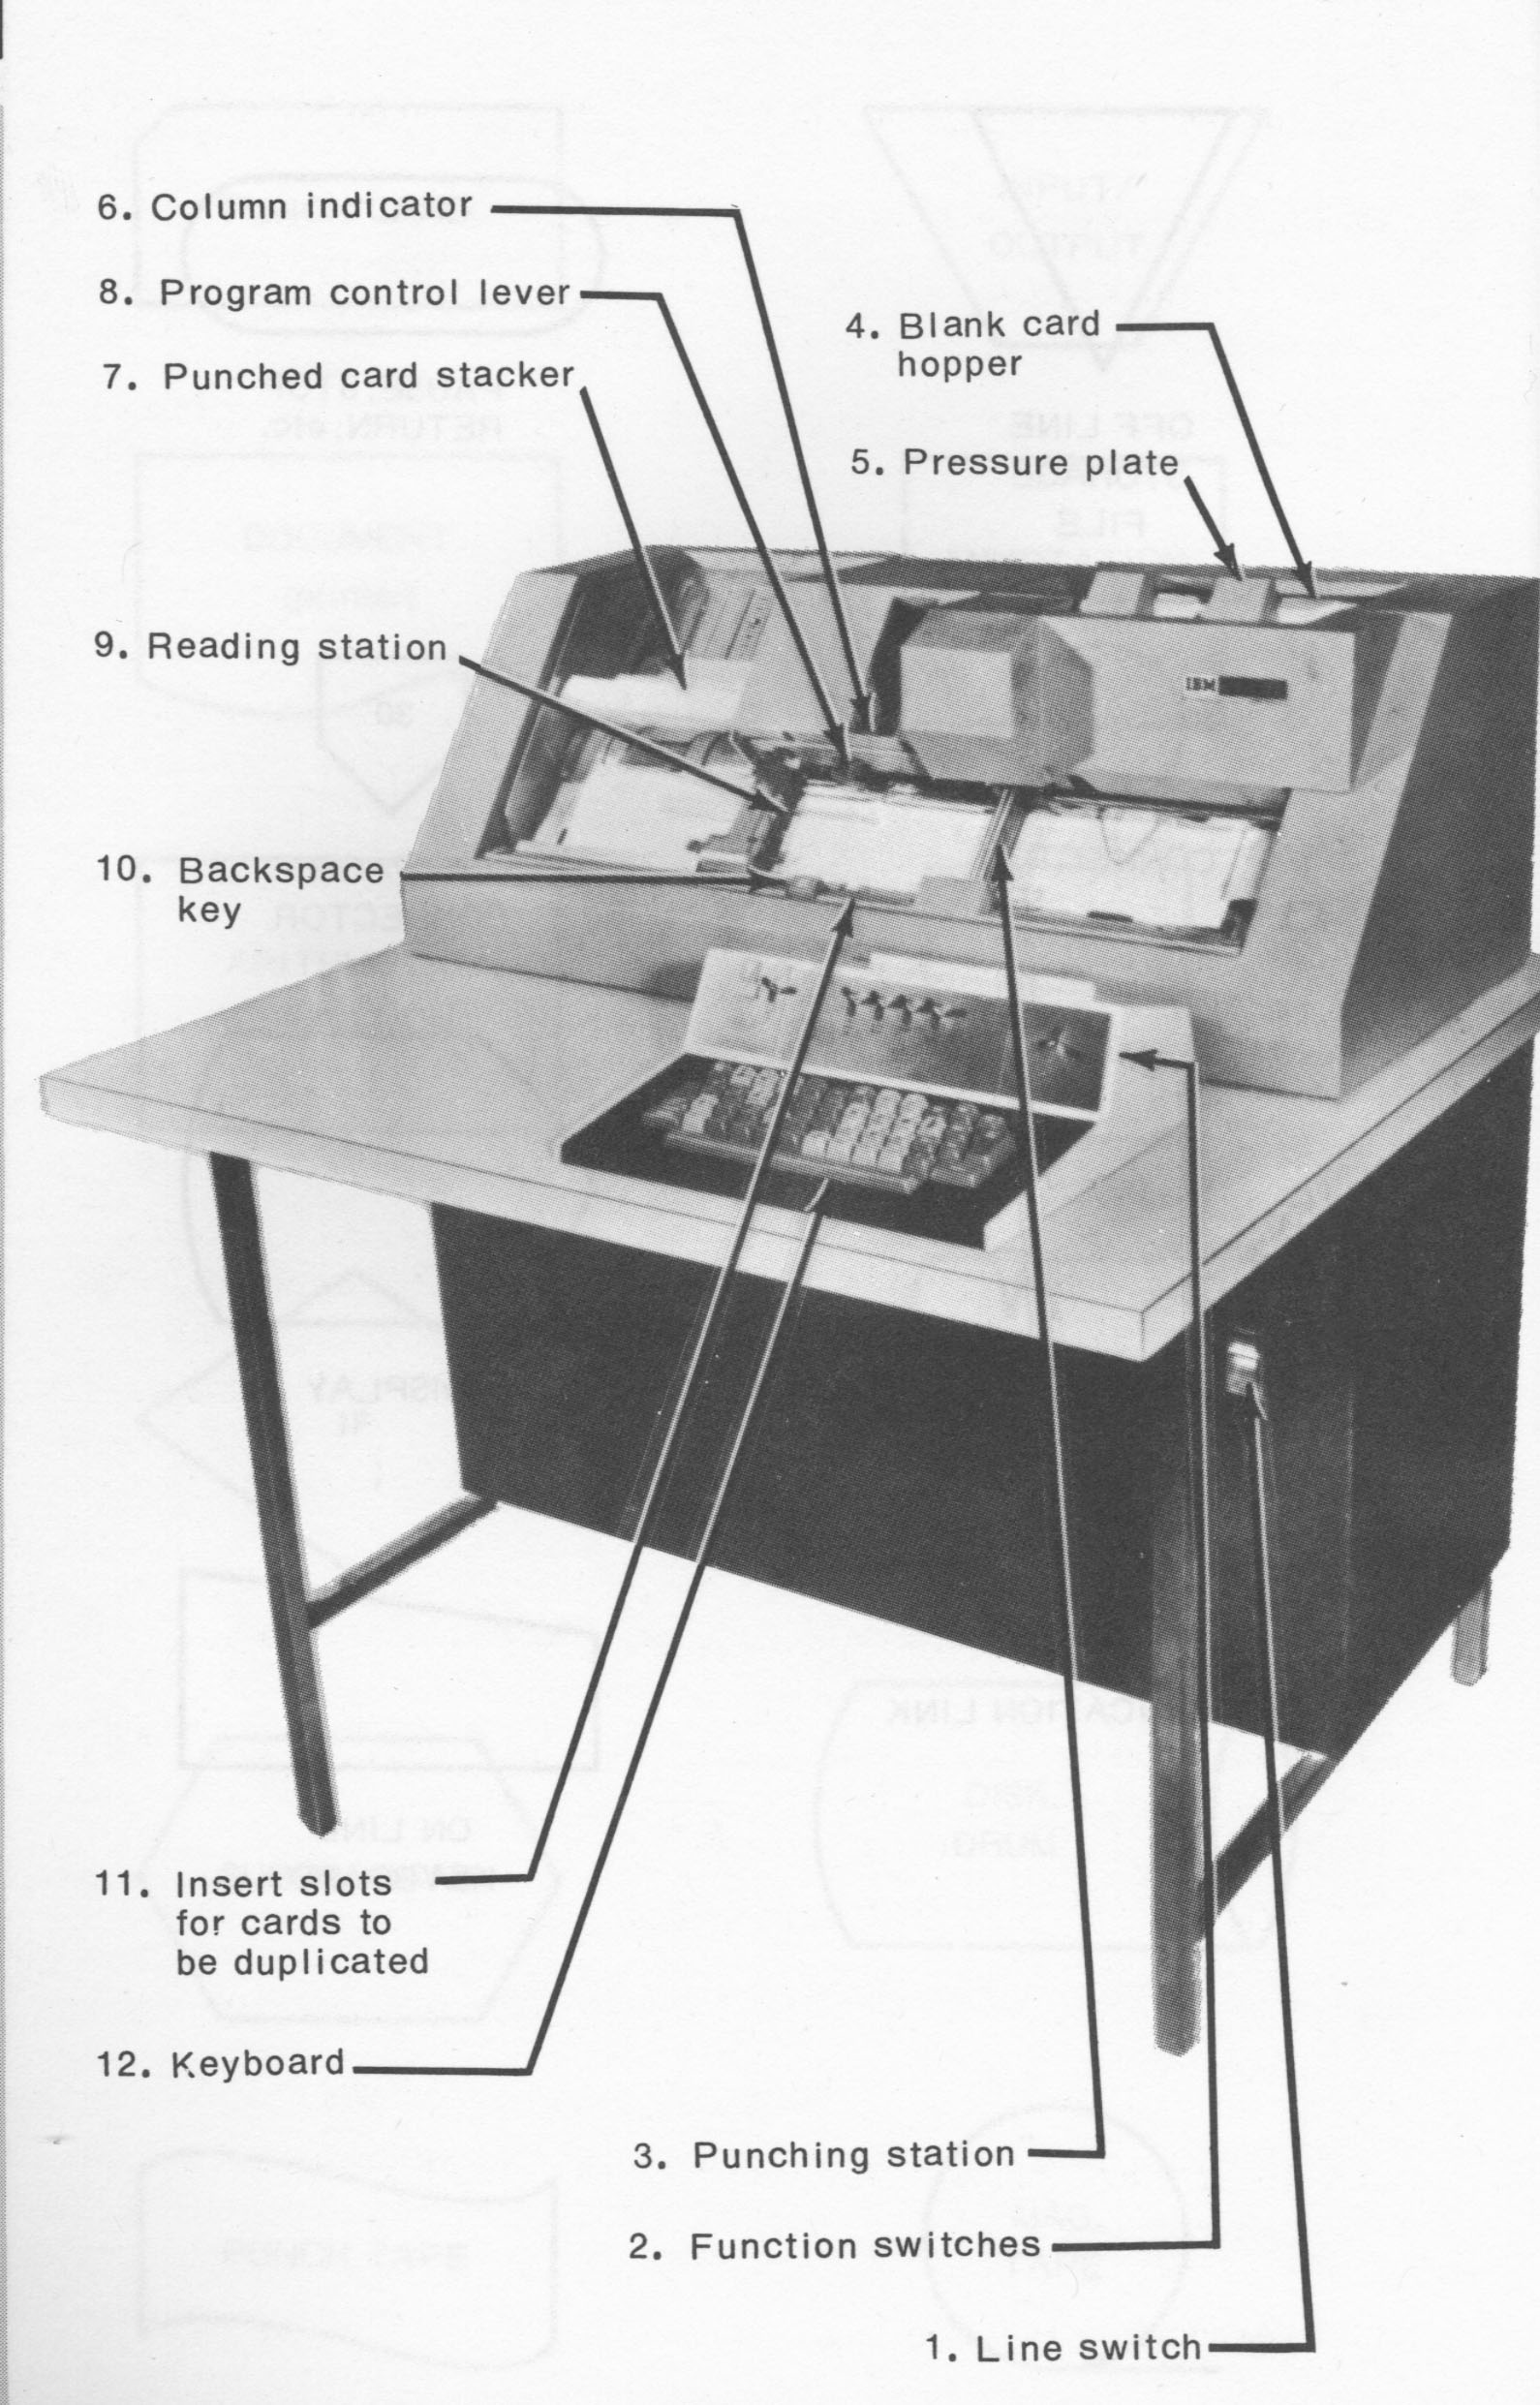
\includegraphics[width=0.8\linewidth]{memoire-images/keypunch.jpg}
\end{center}
(source: \url{http://www.math-cs.gordon.edu/courses/cs323/FORTRAN/keypunch.html})

pour transcrire le programme sur des cartes perforées\footnote{avec 4 perfos, il fallait évidemment faire la queue, un peu moins la nuit et le
week-end}. Chaque carte contenait une ligne de 80 caractères.
\begin{center}
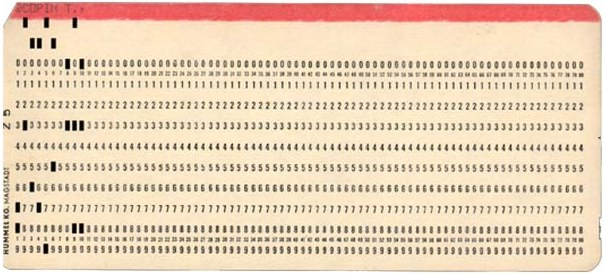
\includegraphics[width=\linewidth]{memoire-images/punch-card.jpg}
\end{center}

\item les cartes, entourées par un élastique, étaient placés dans un
  bac qu'un étudiant (rémunéré) allait porter au Centre de Calcul
  Interuniversitaire, où se trouvait l'ordinateur IRIS 80, trois ou
  quatre fois par jour. Les bacs de cartes étaient alors confiés à un
  opérateur, qui les plaçait dans le lecteur de cartes, lançait le
  traitement et récupérait (bien plus tard) les cartes avec les
  listings de résultats.
\begin{center}
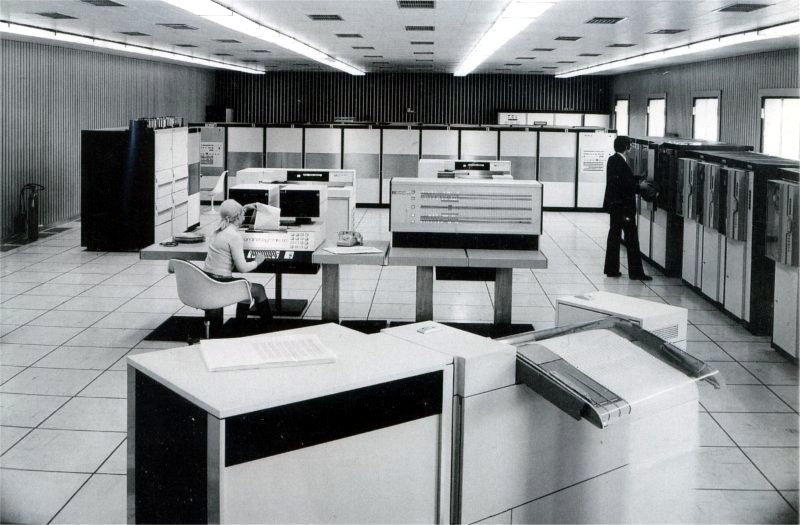
\includegraphics[width=\linewidth]{memoire-images/iris80-1.jpg}
\end{center}
Source \url{http://www.feb-patrimoine.com/projet/iris80/iris80.htm}.


\item il en profitait pour ramener les travaux précédents, avec les
  listings de résultats.
\item en récupérant son travail, l'étudiant constatait généralement
  qu'il manquait un point-virgule quelque part : ne restait plus qu'à trouver où,
  remplacer la carte fautive, et remettre le paquet dans le bac de départ, pour
 avoir le résultat quelques heures plus tard.
\end{enumerate}
Dans ces conditions, il était évidemment préférable de réfléchir
avant de taper, et de se relire soigneusement plusieurs fois avant
de mettre les cartes dans le bac...

Les étudiants de troisième cycle, et les chercheurs en mathématiques
et informatique, disposaient quant à eux d'une petite salle avec
quelques \textbf{terminaux conversationnels} hétéroclites : telex
Olivetti, terminaux à écran cathodiques (HP 2621), clavier avec imprimante
thermique, écran graphique Textronix 4027, reliées directement au
centre de calcul par des lignes à 9600 bit/s. De quoi travailler très confortablement.


\section{Travailler à plusieurs : le temps partagé} 

En effet un nouveau besoin est apparu avec l'utilisation de terminaux
interactifs : telex transformés, machines à écrire électriques, et
écrans alphanumériques.  Au départ les utilisateurs peuvent soumettre
de nouvelles tâches dans le traitement par lots, mais les programmes
interactifs amènent une contrainte supplémentaire : chaque utilisateur
doit avoir l'impression d'utiliser une machine ``réactive'' : si un
collègue lance un programme de calcul lourd (quelques milliers de
décimales de $\pi$)\footnote{ou un programme qui boucle, comme ça
  arrive parfois.}, ça ne doit pas empêcher les autres de travailler
en monopolisant le temps du processeur.


C'est la prise en compte de cette contrainte qui conduit au \emph{time
  sharing} : le temps du processeur est partagé ``équitablement''
entre les utilisateurs.

 
Parmi les premiers systèmes, le plus connu est CTSS (Compatible Time
Sharing System) issu du projet MAC (Multi Access Computer) de John
McCarthy au MIT\footnote{ John McCarthy, décédé en octobre 2011, est
  un des pionniers de l'informatique : systèmes d'exploitation,
  intelligence artificielle, programmation symbolique et
  fonctionnelle, etc. Lire sa biographie sur Wikipedia. Parmi ses
  articles, un mémo ``\emph{A Time Sharing Operator Program for Our
    Projected IBM 709}" daté du 1er janvier 1959.  Voir ses souvenirs
  sur le time-sharing dans
  \url{http://www-formal.stanford.edu/jmc/history/timesharing/timesharing.html}
}.  Ce système multi-utilisateurs (à partir de 1961, en production en
1964) tournait sur un IBM 7094 modifié, avec une mémoire de 2 fois 32K
mots de 36 bits.  Lire par exemple ``\emph{The IBM 7094 and CTSS}''
par Tom Van Vleck, \url{http://www.multicians.org/thvv/7094.html}

\paragraph{A voir absolument : } le reportage  ``\emph{1963 Timesharing: A Solution to Computer
  Bottlenecks}'' (27 minutes) sur
\url{http://www.youtube.com/watch?v=Q07PhW5sCEk}, avec une longue
interview de Fernando J. Corbato, responsable du projet, qui explique le fonctionnement du temps partagé, suivie par
une démonstration.

\begin{center}
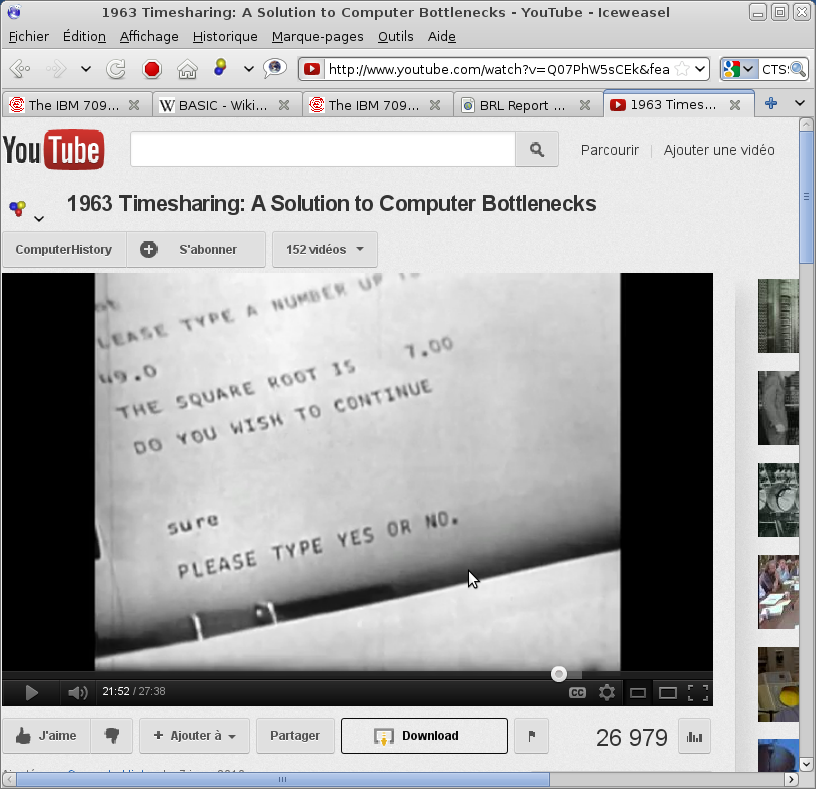
\includegraphics[width=\linewidth]{Videos/corbato-demo.png}
\end{center}


Une démonstration plus courte \url{http://www.youtube.com/watch?v=sjnmcKVnLi0}
 (\emph{Robert Fano explains scientific computing}), à partir de 5:20.



\begin{exercice} Imaginons que 3 utilisateurs d'un système en temps partagé lancent en même
temps des travaux qui nécessitent 10 minutes de calcul chacun.
\begin{enumerate}
\item si ces travaux sont envoyés dans une file d'attente pour être
  traités un par un, le premier utilisateur aura sa réponse dans 10
  minutes, le second dans 20 minutes, et le troisième dans 30, d'où
  un temps d'attente moyen de 20 minutes ;
\item si ils se déroulent en temps partagé, ils dureront tous les trois 30 minutes.
\end{enumerate}
Dans ce contexte, pourquoi les utilisateurs préfèrent-il quand même 
la seconde solution ?
\end{exercice}

\section{De nos jours... }


Les systèmes d'exploitation modernes\footnote{à l'exception de quelques systèmes embarqués ou de super-calculateurs} sont tous capables de faire
exécuter plusieurs tâches en même temps.  Sous Unix, la commande
\texttt{top} vous permet de voir les tâches en cours : sur un
ordinateur personnel vous constaterez qu'il en a au moins une bonne
centaine, plusieurs milliers sur un serveur.

Les solutions qui permettent le fonctionnement en multi-tâches ont été 
trouvées, mises en place et généralisées, dès le début des années 60 :
interruptions, partage de la mémoire, etc.

Dans les années 70 et 80, on a assisté à un recul apparent : les
premiers micro-ordinateurs étaient destinés à un usage personnel. 

Les contraintes de coût qui ne permettaient qu'une faible capacité
mémoire (dizaines ou centaines de kilo-octets) expliquent la
réapparition, pendant une dizaine d'années, des systèmes mono-tâches,
comme CP/M (Kildall, 1977) et MS-DOS (1981).

\begin{exercice}
Avez-vous vraiment besoin d'un système multi-tâches, avec protection
mémoire etc, dans votre smartphone ?
\end{exercice}


\end{multicols}
